% This is "aamas2016_sample.tex", a revised version of aamas2015_sample.tex
% This file should be compiled with "aamas2016.cls"
% This example file demonstrates the use of the 'aamas2015.cls'
% LaTeX2e document class file. It is intended for those submitting
% articles to the AAMAS-2016 conference. This file is based on
% the sig-alternate.tex example file.
% The 'sig-alternate.cls' file of ACM will produce a similar-looking,
% albeit, 'tighter' paper resulting in, invariably, fewer pages
% than the original ACM style.
%
% ----------------------------------------------------------------------------------------------------------------
% This .tex file (and associated .cls ) produces:
%       1) The Permission Statement
%       2) The Conference (location) Info information
%       3) The Copyright Line with AAMAS data
%       4) NO page numbers
%
% as against the acm_proc_article-sp.cls file which
% DOES NOT produce 1) through 3) above.
%
% Using 'aamas2015.cls' you don't have control
% from within the source .tex file, over both the CopyrightYear
% (defaulted to 20XX) and the IFAAMAS Copyright Data
% (defaulted to X-XXXXX-XX-X/XX/XX).
% These information will be overwritten by fixed AAMAS 2015  information
% in the style files - it is NOT as you are used to with ACM style files.
%
% ---------------------------------------------------------------------------------------------------------------
% This .tex source is an example which *does* use
% the .bib file (from which the .bbl file is produced).
% REMEMBER HOWEVER: After having produced the .bbl file,
% and prior to final submission, you *NEED* to 'insert'
% your .bbl file into your source .tex file so as to provide
% ONE 'self-contained' source file.
%


\documentclass{aamas2016}
\usepackage{graphics} % for pdf, bitmapped graphics files
\usepackage{comment}
\usepackage{amsmath,amssymb,amsxtra,amsfonts}%,comment}
% The following packages can be found on http:\\www.ctan.org
\usepackage{graphics} % for pdf, bitmapped graphics files
\usepackage{epsfig} % for postscript graphics files
\usepackage{amsfonts}
\usepackage{url}
\usepackage{color}
\usepackage{threeparttable}
%\usepackage{algorithmic}
\usepackage{algorithmicx}
\usepackage{algpseudocode}
\usepackage{algorithm}

% For algorithms
%\usepackage{algorithm}
%\usepackage{algorithmic}
%\usepackage{hyperref}
%\newcommand{\listspace}{\vspace{0.5em}}
%\newcommand{\theHalgorithm}{\arabic{algorithm}}

% Mathematics
\newcommand{\iforget}{\displaystyle}
\newcommand\Nat{\mathbb{N}}
\renewcommand\natural{\mathbb{N}}
\newcommand\rot{\mathbb{S}}
%% Math defs
% The set of reals, integers, etc.
\renewcommand{\Re}{\mathbb{R}}
\newcommand{\Ze}{\mathbb {Z}}
\newcommand{\Pe}{\mathbb {P}}
\newcommand{\I}{\mathcal{I}}                                                          

% \newcommand{\qed}{\hfill \ensuremath{\Box}}
\newcommand{\blambda}{\boldsymbol\lambda}
\newcommand{\bLambda}{\boldsymbol\Lambda}
\newcommand{\bpsi}{\boldsymbol\psi}
\newcommand{\bPsi}{\boldsymbol\Psi}
\newcommand{\hatE}{\hat{\mathbb{E}}_{N}}
\newcommand{\transpose}{\text{$\mathsf{T}$}}

\newtheorem{proposition}{Proposition}
% \newenvironment{proof}[1][Proof]{\begin{trivlist}
% \item[\hskip \labelsep {\bfseries #1}]}{\end{trivlist}}
\newtheorem{assumption}{Assumption}
\newtheorem{corollary}{Corollary}
\newtheorem{remark}{Remark}
\newtheorem{lemma}{Lemma}

\DeclareMathOperator*{\argmin}{argmin}

% if you are using PDF LaTeX and you cannot find a way for producing
% letter, the following explicit settings may help

\usepackage{pifont}
\newcommand{\note}[3]{{\color{#2} [ \ding{42} \textbf{#1:} {\small #3} ]}}
\newcommand{\comMarcio}[1]{\note{Marcio}{red}{#1}}
\newcommand{\comEric}[1]{\note{Eric}{blue}{#1}}
\newcommand{\comMatt}[1]{\note{Matt}{green}{#1}}
\newcommand{\comJames}[1]{\note{James}{magenta}{#1}}
\newcommand{\comGabe}[1]{\note{Gabe}{cyan}{#1}}

\newcommand{\Task}[1]{\mathcal{Z}^{(#1)}}
\newcommand{\Mt}[1]{\phi\bigl(\mt{#1}\bigr)}
\newcommand{\mt}[1]{\bm{m}^{(#1)}}
\newcommand{\Dt}[1]{D^{(#1)}}
\newcommand{\st}[1]{\bm{s}^{(#1)}}
\newcommand{\sthat}[1]{\hat{\bm{s}}^{(#1)}}
\newcommand{\Th}[1]{\bm{\theta}^{(#1)}}
\newcommand{\At}[1]{\bm{\alpha}^{(#1)}}
\newcommand{\ComboVec}[1]{\bm{\beta}^{(#1)}}
\newcommand{\ComboDict}{\bm{K}}
\newcommand{\xit}[2]{\bm{x}_{#1}^{(#2)}}
\newcommand{\Xt}[1]{X^{(#1)}}
\newcommand{\yit}[2]{y_{#1}^{(#2)}}
\newcommand{\yt}[1]{\bm{y}^{(#1)}}
\newcommand{\pairsim}[1]{d(#1)}
\newcommand{\learned}[1]{h\Big( \pairsim{#1},\phi \Big)} %\tilde{p(#1)}
\newcommand{\pairset}[1]{\bm{D}_{#1}}
\newcommand{\learnedset}[1]{\bm{D}_{#1}'}
\newcommand{\reveng}[1]{R(#1)}
%\newcommand{\argmin}{\arg\!\min}
\newcommand{\Tau}{|\mathbf{T}|} 


\usepackage{bm}
%\usepackage{mathrsfs}

\usepackage{xspace}
\newcommand{\etal}{et~al.\xspace} 

\pdfpagewidth=8.5truein
\pdfpageheight=11truein

\begin{document}

% In the original styles from ACM, you would have needed to
% add meta-info here. This is not necessary for AAMAS 2015  as
% the complete copyright information is generated by the cls-files.


\title{{\color{red} Lifelong Learning for Disturbance Rejection on Mobile Robots} }

% AUTHORS


% For initial submission, do not give author names, but the
% tracking number, instead, as the review process is blind.

% You need the command \numberofauthors to handle the 'placement
% and alignment' of the authors beneath the title.
%
% For aesthetic reasons, we recommend 'three authors at a time'
% i.e. three 'name/affiliation blocks' be placed beneath the title.
%
% NOTE: You are NOT restricted in how many 'rows' of
% "name/affiliations" may appear. We just ask that you restrict
% the number of 'columns' to three.
%
% Because of the available 'opening page real-estate'
% we ask you to refrain from putting more than six authors
% (two rows with three columns) beneath the article title.
% More than six makes the first-page appear very cluttered indeed.
%
% Use the \alignauthor commands to handle the names
% and affiliations for an 'aesthetic maximum' of six authors.
% Add names, affiliations, addresses for
% the seventh etc. author(s) as the argument for the
% \additionalauthors command.
% These 'additional authors' will be output/set for you
% without further effort on your part as the last section in
% the body of your article BEFORE References or any Appendices.

%\numberofauthors{8} %  in this sample file, there are a *total*
% of EIGHT authors. SIX appear on the 'first-page' (for formatting
% reasons) and the remaining two appear in the \additionalauthors section.
%

\numberofauthors{7}

% \author{
% % You can go ahead and credit any number of authors here,
% % e.g. one 'row of three' or two rows (consisting of one row of three
% % and a second row of one, two or three).
% %
% % The command \alignauthor (no curly braces needed) should
% % precede each author name, affiliation/snail-mail address and
% % e-mail address. Additionally, tag each line of
% % affiliation/address with \affaddr, and tag the
% % e-mail address with \email.
% % 1st. author
% David Isele\\
% % 2nd. author
% \alignauthor
% Jos\'e Marcio Luna\\
% % 3rd. author
% \alignauthor Eric Eaton
% \and  % use '\and' if you need 'another row' of author names
% \alignauthor
% \affaddr{University of Pennsylvania}\\
%       \affaddr{3330 Walnut St}\\
%       \affaddr{Philadelphia, PA 19104}\\
%       \email{\{isele,joseluna,eeaton\}@seas.upenn.edu}
% \and
% \alignauthor Gabriel de la Cruz\\
% % 5th. author
% \alignauthor James Irwin\\
% % 6th. author
% \alignauthor Brandon Kallaher\\
% % 7th. author
% \alignauthor Matthew Taylor\\
% \and
% \alignauthor
%       \affaddr{Washington State University}\\
%       \affaddr{P.O. Box 642752}\\
%       \affaddr{Pullman, WA 99164}\\
%       \email{\{gabriel.delacruz,james.irwin,brandon.kallaher.taylor\}@wsu.edu}
% }


\author{
% You can go ahead and credit any number of authors here,
% e.g. one 'row of three' or two rows (consisting of one row of three
% and a second row of one, two or three).
%
% The command \alignauthor (no curly braces needed) should
% precede each author name, affiliation/snail-mail address and
% e-mail address. Additionally, tag each line of
% affiliation/address with \affaddr, and tag the
% e-mail address with \email.
% 1st. author
\hspace{-1.5em} David Isele\\
\hspace{-1.5em} \affaddr{Univ.~of Pennsylvania}\\
\hspace{-1.5em} \email{\affaddr{isele@seas.upenn.edu}}
% 2nd. author
\alignauthor
Jos\'e Marcio Luna\\
\affaddr{Univ.~of Pennsylvania}\\
      \email{\affaddr{joseluna@seas.upenn.edu}}
% 3rd. author
\alignauthor Eric Eaton\\
\affaddr{Univ.~of Pennsylvania}\\
\email{\affaddr{eeaton@seas.upenn.edu}}
% use '\and' if you need 'another row' of author names
% 4th. author
\alignauthor Gabriel de la Cruz\\
      \affaddr{Washington State Univ.}\\
      \email{\affaddr{gabriel.delacruz@wsu.edu}}
 \and
% 5th. author
\alignauthor James Irwin\\
      \affaddr{Washington State Univ.}\\
      \email{\affaddr{james.irwin@wsu.edu}}
% 6th. author
\alignauthor Brandon Kallaher\\
      \affaddr{Washington State Univ.}\\
      \email{\affaddr{brandon.kallaher@wsu.edu}}
% 7th. author
\alignauthor Matthew E.~Taylor\\
      \affaddr{Washington State Univ.}\\
      \email{\affaddr{taylorm@eecs.wsu.edu}}
}

%\and
%% 7th. author
%\alignauthor Lawrence P. Leipuner\\
%       \affaddr{Brookhaven Laboratories}\\
%       \affaddr{Brookhaven National Lab}\\
%       \affaddr{P.O. Box 5000}\\
%       \email{lleipuner@researchlabs.org}

%% 8th. author
%\alignauthor Sean Fogarty\\
%       \affaddr{NASA Ames Research Center}\\
%       \affaddr{Moffett Field}\\
%       \affaddr{California 94035}\\
%       \email{fogartys@amesres.org}

%% 9th. author
%\alignauthor Charles Palmer\\
%       \affaddr{Palmer Research Laboratories}\\
%       \affaddr{8600 Datapoint Drive}\\
%       \affaddr{San Antonio, Texas 78229}\\
%       \email{cpalmer@prl.com}

%}


% \alignauthor
% Paper XXX
%Ben Trovato\titlenote{Dr.~Trovato insisted his name be first.}\\
%       \affaddr{Institute for Clarity in Documentation}\\
%       \affaddr{1932 Wallamaloo Lane}\\
%       \affaddr{Wallamaloo, New Zealand}\\
%       \email{trovato@corporation.com}
% 2nd. author
%\alignauthor
%G.K.M. Tobin\titlenote{The secretary disavows any knowledge of this author's actions.}\\
%       \affaddr{Institute for Clarity in Documentation}\\
%       \affaddr{P.O. Box 1212}\\
%       \affaddr{Dublin, Ohio 43017-6221}\\
%       \email{webmaster@marysville-ohio.com}
% 3rd. author
%\alignauthor Lars Th{\o}rv{\"a}ld\titlenote{This author is the one who did all the really hard work.}\\
%       \affaddr{The Th{\o}rv{\"a}ld Group}\\
%       \affaddr{1 Th{\o}rv{\"a}ld Circle}\\
%       \affaddr{Hekla, Iceland}\\
%       \email{larst@affiliation.org}
% }

%\and  % use '\and' if you need 'another row' of author names

% 4th. author
%\alignauthor Lawrence P. Leipuner\\
%       \affaddr{Brookhaven Laboratories}\\
%       \affaddr{Brookhaven National Lab}\\
%       \affaddr{P.O. Box 5000}\\
%       \email{lleipuner@researchlabs.org}

% 5th. author
%\alignauthor Sean Fogarty\\
%       \affaddr{NASA Ames Research Center}\\
%       \affaddr{Moffett Field}\\
%       \affaddr{California 94035}\\
%       \email{fogartys@amesres.org}

% 6th. author
%\alignauthor Charles Palmer\\
%       \affaddr{Palmer Research Laboratories}\\
%      \affaddr{8600 Datapoint Drive}\\
%       \affaddr{San Antonio, Texas 78229}\\
%       \email{cpalmer@prl.com}

%\and

%% 7th. author
%\alignauthor Lawrence P. Leipuner\\
%       \affaddr{Brookhaven Laboratories}\\
%       \affaddr{Brookhaven National Lab}\\
%       \affaddr{P.O. Box 5000}\\
%       \email{lleipuner@researchlabs.org}

%% 8th. author
%\alignauthor Sean Fogarty\\
%       \affaddr{NASA Ames Research Center}\\
%       \affaddr{Moffett Field}\\
%       \affaddr{California 94035}\\
%       \email{fogartys@amesres.org}

%% 9th. author
%\alignauthor Charles Palmer\\
%       \affaddr{Palmer Research Laboratories}\\
%       \affaddr{8600 Datapoint Drive}\\
%       \affaddr{San Antonio, Texas 78229}\\
%       \email{cpalmer@prl.com}

%}

%% There's nothing stopping you putting the seventh, eighth, etc.
%% author on the opening page (as the 'third row') but we ask,
%% for aesthetic reasons that you place these 'additional authors'
%% in the \additional authors block, viz.
%\additionalauthors{Additional authors: John Smith (The Th{\o}rv{\"a}ld Group,
%email: {\texttt{jsmith@affiliation.org}}) and Julius P.~Kumquat
%(The Kumquat Consortium, email: {\texttt{jpkumquat@consortium.net}}).}
%\date{30 July 1999}
%% Just remember to make sure that the TOTAL number of authors
%% is the number that will appear on the first page PLUS the
%% number that will appear in the \additionalauthors section.

\maketitle

\begin{abstract}
Learning controllers for multiple systems is often an expensive process when controllers for each system are learned individually. Advances in lifelong learning suggest that information between systems can be shared, improving the quality of the controllers that are learned. However these results have been largely theoretical, with applications limited to benchmark problems with known dynamics. We show that these methods can be extended to robotic platforms. Particularly we validate our assumptions for transfer learning between tasks with unknown dynamics in order to carry out a disturbance rejection problem. We view this as early work leading up to learning robust fault tolerant control.

\end{abstract}

% Note that the category section should be completed after reference to the ACM Computing Classification Scheme available at
% http://www.acm.org/about/class/1998/.

\category{I.2.6}{Artificial Intelligence}{Learning}
\category{I.2.9}{Artificial Intelligence}{Robotics}

%A category including the fourth, optional field follows...
%\category{D.2.8}{Software Engineering}{Metrics}[complexity measures, performance measures]

%General terms should be selected from the following 16 terms: Algorithms, Management, Measurement, Documentation, Performance, Design, Economics, Reliability, Experimentation, Security, Human Factors, Standardization, Languages, Theory, Legal Aspects, Verification.

\terms{algorithms, experimentation}

%Keywords are your own choice of terms you would like the paper to be indexed by.

\keywords{lifelong learning, policy gradients, reinforcement learning, robotics}


\section{Introduction}

%{\color{red} Organization:

%1. Control system theory(Model approach)\\
%2. Model-free approach\\
%4. Gazebo model not really available\\
%3. Connection Lifelong Learning: fault tolerant in multi-agent systems disturbance rejection as preliminary step
%4. Initial experiments constant and unknown disturbances\\
%6. Turtlebot and Quadcopter experiments with linear and nonlinear policies\\
%5. Learning in simulation and then physical robots}


%
%In control systems, a perfect model of the dynamics of the system is often necessary to guarantee the stabilization of the system. 
%This can be problematic in complicated systems where the dynamics are difficult to model or require information that is not available to 
%the designer \cite{Khalil-2002,Tempo-2013}. %such as failures that change dynamics.

In control systems, a perfect model of the dynamics of the system is often necessary to guarantee the stabilization of the system. This can be problematic in complicated systems where the dynamics are difficult to model or require information that is not available to the designer. %such as failures that change dynamics.


% VIEW MODEL FREE AS LIFELONG LEARNING
Policy search approaches have been proposed to deal with the design of controllers in model-free applications.
However, it is difficult to make claims of robustness or generalization of the learned controllers 

Our goal is to learn fault tolerant control in multi-agent systems. In order to approach this problem we begin by developing a method that can accomplish disturbance rejection across multiple robots. 
%Given differences in manufacturing and wear, even identically designed robots may require very different control policies. % very robustness as many different systems
%This motivates us to phrase the problem of learning robust controllers that reject disturbances as a multi-system problem.
Given a collection of robots each with a different unknown disturbance, learning a unique control policy for each robot in the system can be very costly. One approach to reduce the amount of learning is to share information between robots. 

Lifelong learning \cite{Ruvolo2013} is a promising approach for accomplishing information sharing between different robots. It works on-line, allowing the different systems to be encountered consecutively so \textit{a priori} knowledge of all the different systems is not required at the start of training. It also preserves and possibly improves the models encountered early on, in contrast to transfer methods which only optimize performance on the target system.

However most recent work in lifelong learning \cite{Ruvolo2013,BouAmmar2014a,bouAmmar2015unsupervised} has been theoretical, using simulations of benchmark problems with known dynamics to demonstrate knowledge sharing. The contribution of this work is to present the first results of lifelong learning on robotic systems. We do this by applying the PG-ELLA framework \cite{BouAmmar2014a} to the problem of disturbance rejection on a set of Turtlebots in Gazebo Simulator. In this work in progress, the obtained results motivate future experiments on the real robot. 

After discussing related work in section \ref{related}, we review policy gradients and describe the particular base-learner we are using for lifelong learning in  section \ref{background}. We then outline our experiments in section \ref{Experiments}, showing how lifelong learning can be used to accomplish disturbance rejection on robotic systems.

% Learning on robotic systems is a very costly process. The time needed to run learning algorithms often prohibits running the large number of trials needed to learn a robust model. %, and physical systems wear down from repeated trials often changing the system over time. This problem is greatly exacerbated in multi-robot systems which can contain many possibly different systems, each of  which may have a different objective, and therefore may require learning a unique controller for each agent in the system.


%Work in multi-task learning has shown that performance can be improved by sharing data between tasks. Recent advances in lifelong learning show that knowledge sharing can be handled efficiently in an on-line manner, re\cite{Ruvolo2013}moving the restriction that data be collected for all tasks before optimization can take place. However these methods are often demonstrated on simulated systems with known dynamics and parameterizations. 

%transfer citations \cite{barrett2010transfer} \cite{chalup2007machine}


% We propose a lifelong learning method that can learn controllers in the presence of unknown disturbances that differ from task to task. Unlike most previous work in lifelong learning, we demonstrate this method on Turtlebots, an affordable robotics platform.  

\section{Related work}\label{related}

% CURRENT CONTROL STATE OF THE ART
Building mathematical models that describe the behavior of physical systems is common practice to analyze, predict and 
control their behavior to fulfill specific goals. Well known techniques for modeling physical systems include partial, ordinary
differential and difference equations \cite{Khalil-2002,Nise-2010}, and Discrete Event Systems (DES) such as queueing and Petri networks 
\cite{Cassandras-2008,Luna-2015,Urgaonkar-2007}.\comJames{This list of modeling techniques might want to get reworded}
Control systems theory uses differential and difference equations to model the mechanics of physical systems. In control systems
a validated model provides ways of assessing the stability and stabilizability of the system to be able to control its behavior.

Some of the typical problems in control systems are regulation, trajectory tracking, disturbance rejection and
robustness among many others \cite{Khalil-2002, Lewis-2012,Nise-2010}. All these problems are associated with the analysis of the stabilizability of the system, 
as well as the design of controllers to stabilize it. These controllers consist of theoretical artifacts that would allow 
the solution of control problems such as the aforementioned ones. 

% DISTURBANCE REJECTION
The disturbance rejection problem consists of implementing a controller that allows the plant to fulfill the desired task while compensating
for a disturbance that modifies its nominal dynamics. As long as there is an accurate model of the plant, several mathematical
artifacts have been provided to handle constant, constant and unknown, time-varying and even stochastic disturbances 
\cite{Dorato-2000,Khalil-2002,Lewis-2012}. 
However, things get more complicated when no model is provided, even for simple disturbances. In a model-free setting, the goal is to design a 
controller that stabilizes a system whose model is not available due to complex internal iterations, uncertainty in the system, event-based
dynamics and technological limitations. Unlike typical control system theory where policies are generated from a model, we generate policies based on sampled trajectories generated by simulation.

% RL methods
%pilco model based but learns the model \cite{deisenroth2011pilco}
Reinforcement learning \cite{kober2013reinforcement} is often utilized to learn controllers in a model-free settings. Amongst reinforcement learning algorithms, policy gradient (PG) methods \cite{sutton1999policy,williams1992simple} are popular in robotic applications \cite{kober2009policy,peters2008natural} since they accommodate continuous state/action spaces and can scale well to high dimensional spaces. Different from these works we use policy gradients in a lifelong learning setting.

%Examples exist that do not explicitly compute gradients (episodic REINFORCE)~\cite{williams1992simple}, specialized to dynamic motor primitives PoWER~\cite{kober2009policy}, and , use natural gradients Natural Actor Critic~\cite{peters2008natural})

% RL to LL
It has been shown that PG methods can be used in a lifelong learning setting \cite{BouAmmar2014a,bouAmmar2015unsupervised}, however these works focus largely on theory, using benchmark simulations to demonstrate their results. While there are examples of lifelong learning on robots, they tend to focus in skill refinement on a single robot \cite{kleiner2002towards,thrun1995lifelong} rather than sharing information across multiple robots as we do in our work. 



\section{Background} \label{background}
Our approach works by sharing knowledge between different robotic systems. The policy for each system is learned by reinforcement learning. In this section we cover the mathematical framework that supports our experiments on lifelong learning.

\subsection{Reinforcement Learning}

A reinforcement learning (RL) agent must select sequential actions to maximize its expected return. RL approaches do not 
require previous knowledge of the system dynamics, instead, the control policies are learned through the interactions with the system.
RL problems are typically formalized as Markov Decision Processes (MDPs) with the form $\langle \mathcal{X}, \mathcal{A}, P, R, \gamma \rangle$ where
$\mathcal{X}\subset\Re^{d_{x}}$ is the set of states, $\mathcal{A}$ is the set of actions, 
$P:\mathcal{X}\times \mathcal{A}\times \mathcal{X}\rightarrow [0,1]$ is the state transition probability describing the systems dynamics,
$R:\mathcal{X}\times \mathcal{A} \rightarrow \Re$ is the reward function and $\gamma \in [0,1)$ is the reward discount factor. At each time 
step $h$, the agent is in the state $\mathbf{x}_{h} \in \mathcal{X}$ and must choose an action $\mathbf{a}_{h} \in \mathcal{A}$ so that
it transitions to a new state $\mathbf{x}_{h+1}$ with state transition probability 
$P(\mathbf{x}_{h+1}|\mathbf{x}_{h},\mathbf{a}_{h})$, yielding 
a reward $r_{h}$ according to $R$. The action is selected according to a policy $\pi:\mathcal{X}\times \mathcal{A} \rightarrow [0,1]$ which
specifies a probability distribution over actions given the current state. The goal of RL is to find the optimal policy $\pi^{*}$ 
that maximizes the expected reward.

We use a class of RL algorithms known as Policy Gradient (PG) methods \cite{sutton1999policy}, which are particularly well suited for solving high dimensional problems with continuous state and action spaces, such as robotic control \cite{peters2008natural}. %PG methods are appealing for their ability to handle continuous state and action spaces, as well as their ability to scale well to high dimensions. 

The goal of PG is to use gradient steps to optimize the expected average return:
\begin{equation}
 \mathcal{J}(\boldsymbol{\theta})=\int_{\mathbb{T}}p_{\boldsymbol{\theta}}(\tau)\mathcal{R}(\tau)\mbox{d}\tau,
 \label{retPG}
\end{equation}
where $\mathbb{T}$ is the set of all trajectories and $\mathcal{R}(\tau)$ is the average per-step reward, specifically:
\begin{eqnarray}
 p_{\boldsymbol{\theta}} & = & \prod_{h=0}^{H}p(\mathbf{x}_{h+1}|\mathbf{x}_{h},\mathbf{a}_{h})\pi(\mathbf{a}_{h},\mathbf{x}_{h})  \enspace, \nonumber \\
 \mathcal{R}(\tau) & = & \frac{1}{H}\sum_{h=0}^{H} r(\mathbf{s}_{h},\mathbf{a}_{h},\mathbf{s}_{h+1})  \enspace. \nonumber
\end{eqnarray}

%%\mbox{$
%\begin{equation} \label{pgreturn}
%	\mathcal{J}(\bm{\theta}) = E \left[ \frac{1}{H} \sum_{h=1}^H r_h \right] = \int_{\mathbb{T}} p_{\bm{\theta}}(\bm{\tau})\mathfrak{R}(\bm{\tau})d\bm{\tau}
%%$}, 
%\end{equation}
%where $\mathbb{T}$ is the set of all possible trajectories. $\mathfrak{R}(\bm{\tau}) $ is the average reward for a particular trajectory $\bm{\tau}$
%% is given by \mbox{$\mathfrak{R}(\bm{\tau}) = \frac{1}{H}\sum_{h=1}^{H} r_h$}, 
%and $p_{\bm{\theta}}(\bm{\tau})$ is the probability of $\bm{\tau}$ under an initial state distribution $P_0:\mathcal{X} \mapsto [0,1]$ and following policy $\pi_{\bm{\theta}}$.
%% $p_{\bm{\theta}}(\bm{\tau}) = P_0(\bm{x}_1) \prod_{h=1}^{H} p(\bm{x}_{h+1} \mid \bm{x}_{h},\bm{a}_{h}) \ \pi(\bm{a}_h \mid \bm{x}_{h})$} is the probability of $\bm{\tau}$ under an initial state distribution $P_0:\mathcal{X} \mapsto [0,1]$. 
Most PG methods (e.g. episodic REINFORCE \cite{williams1992simple}, Natural Actor 
Critic \cite{peters2008natural}, and PoWER \cite{kober2009policy}) optimize the policy by maximizing a lower bound on the return, 
comparing trajectories generated by different candidate policies $\pi$. 
In this particular application, the PG method we use in our experiments is finite differences (FD) \cite{Bagnell-2013} 
which optimizes the return directly.

\subsection{Finite Differences for Policy Search}
The local optimization around an existing policy $\pi$ parameterized by a parameter matrix $\boldsymbol{\theta}$ 
is carried out by computing changes in the policy parameters $\boldsymbol{\Delta \theta}$ that will increase the expected reward, thus
producing the iterative update,
\begin{displaymath}
 \boldsymbol{\theta}_{m+1} = \boldsymbol{\theta}_{m}+\boldsymbol{\Delta \theta}_{m}.
\end{displaymath}

%{\color{red}More methods to be added here taken from the survey paper. It might be better to add them to the related work section.}

Gradient-based methods for policy updates follow the gradient of the expected return $\mathcal{J}$ %{\color{red}check the notation for the return and the difference between return and reward} 
given a step-size $\delta$,
\begin{displaymath}
 \boldsymbol{\theta}_{m+1} = \boldsymbol{\theta}_{m}+\delta\nabla_{\boldsymbol{\theta}}\mathcal{J}.
\end{displaymath}

In FD gradients, we have a set of $n$ perturbed policy parameters which are used to estimate the effect of a change in policy parameters:
\begin{displaymath}
 \Delta\hat{\mathcal{J}}_{\mathbf{p}} \approx \mathcal{J}(\boldsymbol{\theta}_{m}+\boldsymbol{\Delta\theta_{p}}) - \mathcal{J}_{ref},
\end{displaymath}
where $\boldsymbol{\Delta\theta_{p}}$ are the individual perturbations for $\mathbf{p}=[1,\ldots,n]$, $\Delta\hat{\mathcal{J}}_{\mathbf{p}}$ is the estimate of their 
effect on the return, and the $\mathcal{J}_{ref}$ is a reference return which is usually taken as the return of the unperturbed
parameters. By using linear regression we get an approximation of the gradient,
\begin{displaymath}
 \nabla_{\boldsymbol{\theta}}\mathcal{J} \approx \left(\boldsymbol{\Delta\Theta^{\transpose}\Delta\Theta}\right)^{-1}\boldsymbol{\Delta\Theta}^{\transpose}\Delta\boldsymbol{\hat{J}_{p}},
\end{displaymath}
where $\Delta\boldsymbol{\hat{J}_{p}}$ contains all the stacked samples of $\Delta\hat{\mathcal{J}}_{\mathbf{p}}$ and  $\boldsymbol{\Delta\Theta}$
contains the stacked perturbations $\boldsymbol{\Delta\theta_{p}}$. This approach is sensitive to the type and magnitude of the perturbations, as well as
to the step size $\delta$. Since the number of perturbations needs to be as large as the number of parameters, this method is
considered to be noisy and inefficient for problems with large sets of parameters.%However since it optimizes the expected return directly, it can potentially learn better policies than methods that optimize a bound that isn\rq{}t tight.

In our experiments, the policy is represented as a function defined over a parameter matrix 
$\boldsymbol{\theta} \in \Re^{d_{\theta}}$. 
Our goal is to optimize the expected average return of Equation \ref{retPG}.


In order to share information across different learned policies, we incorporate the PG learning process into a lifelong machine learning 
setting.

%This average return is common in Policy Gradient (PG) methods \cite{peters2006policy}.  
%The optimization of the policy is carried out by comparing trajectories generated by a policy $\pi_{\boldsymbol{\theta}}$ with those
%generated by a new policy $\pi_{\boldsymbol{\tilde{\theta}}}$. For more details see \cite{TODO}.




\subsection{Lifelong Machine Learning}


Lifelong learning focuses on learning a set of tasks consecutively while performing well across all tasks. Given a round $t = 1,\dots,T$ a task $Z^{(t)}$ is observed. %\comEric{Please don't change notation between papers unless absolutely necessary.  Let's use the exact same notation as in the recent IJCAI paper.} 
In our setting, each task corresponds to a reinforcement learning problem for an individual robot. We assume that the model associated to $Z^{(t)}$ is parameterized by a parameter $\boldsymbol{\theta}^{(t)} \in \Re^{d_{\theta_{t}}}$. The ideal goal is that prior knowledge about tasks $Z^{(1)},\ldots,Z^{(t-1)}$ should provide enough information so that the lifelong learning algorithm performs better and faster on $Z^{(t)}$ while being able to scale as the number of tasks increases.

Following work in both multi-task \cite{Kumar-2012} and lifelong learning \cite{Ruvolo2013}, we assume there is a shared basis $\boldsymbol{L}\in \Re^{d_{x}\times k}$ and a sparse weight vector $\boldsymbol{s}^{(t)}\in \Re^{\l}$, so that the policy parameters $\boldsymbol{\theta}^{(t)}$
are given by,
\begin{displaymath}
 \boldsymbol{\theta}^{(t)}=\boldsymbol{Ls}^{(t)}.
\end{displaymath}

Using the return function in (\ref{retPG}) we propose the following multi-task objective function,
\begin{displaymath}
 \argmin_{\boldsymbol{L},\boldsymbol{S}}\frac{1}{T}\sum_{t}\left[ -\mathcal{J}(\boldsymbol{\theta}^{(t)}) + \lambda \| \boldsymbol{s}^{(t)} \|_{1} \right] + \mu\|\boldsymbol{L}\|_{F}^{2},
\end{displaymath}
where $\boldsymbol{S}$ is the set of the sparse vectors $\boldsymbol{s}^{(t)}$, the L1 norm of $\| \boldsymbol{s}^{(t)} \|_{1}$ 
provides sparse code for $\boldsymbol{s}^{(t)}$ and the Frobenious norm in $\|\boldsymbol{L}\|_{F}^{2}$ provides regularization of $\mathbf{L}$. The
coefficients $\mu$ and $\lambda \in \Re$ are weights for the regularization and sparsity respectively.
The learning objective function is approximated by a second order Taylor expansion around an estimate $\boldsymbol{\alpha}^{(t)}$ of
the single task policy parameters of task $t$. The optimization
problem is solved by using the on-line ELLA algorithm introduced in \cite{Ruvolo2013} and extended to reinforcement 
learning in \cite{BouAmmar2014a}. The optimization problem is solved by incrementally updating $\mathbf{L}$ by the following the
update equations,
%\begin{eqnarray}
\begin{equation}
\begin{array}{r@{}l}
 \boldsymbol{s}^{(t)}  \leftarrow&  \arg\min_{\boldsymbol{s}} \left\| \boldsymbol{\alpha}^{(t)}-\boldsymbol{L}\boldsymbol{s}^{(t)}\right\|_{\boldsymbol{\Gamma}^{(t)}}^{2} + \mu\left\|\boldsymbol{s}\right\|_{1} \enspace, \\%\nonumber \\
 A  \leftarrow & A + \left(\boldsymbol{s}^{(t)}\boldsymbol{s}^{(t)\transpose} \right) \otimes \boldsymbol{\Gamma}^{(t)} \enspace, \\%\nonumber \\
 b  \leftarrow &b + \mbox{vec}\left(  \boldsymbol{s}^{(t)} \otimes \left( \boldsymbol{\theta}^{(t)\transpose}\boldsymbol{\Gamma}^{(t)} \right) \right) \enspace, \\%\nonumber \\
 L \leftarrow& \mbox{mat} \left( \left( \frac{1}{T}\boldsymbol{A} + \lambda\boldsymbol{I}_{l \times d_{\theta},l \times d_{\theta} }\right)^{-1} \frac{1}{T}\boldsymbol{b} \right) \enspace. %\nonumber
 \label{onlineupdate}
\end{array}
\end{equation}
%\end{eqnarray}


where $\|\boldsymbol{v}\|_{\boldsymbol{A}}^{2}=\boldsymbol{v}^{\transpose}\boldsymbol{A}\boldsymbol{v}$ and $\boldsymbol{\Gamma}^{(t)}$ is 
the Hessian of the PG objective function, and $\boldsymbol{A}$ and $\boldsymbol{b}$ are initialized to zero matrices. The full algorithm is described in Algorithm \ref{algo:PGELLA}.

%Notice that PG relies on the indirect maximization of the return function based on the maximization of a lower bound. Although this bound has reportedly been tight enough to guarantee maximization of the return function, we chose to use finite differences to search the optimal policy to make sure we maximize the return function directly.

%\begin{algorithm}[t]
%\caption{$\mbox{PG-ELLA}\left (k,\lambda,\mu \right)$\label{alg:PGELLA}}          % give the algorithm a caption
%\begin{algorithmic}
%\STATE $T \gets 0$, \enspace $\mathbf{A}\gets \mbox{\textbf{zeros}}_{k\times d,k \times d}$,
%\STATE $\mathbf{b} \gets \mbox{\textbf{zeros}}_{k\times d,1}$, \enspace $\mathbf{L} \gets \mbox{\textbf{zeros}}_{d,k}$%	 \COMMENT{$\mathbf{\mbox{\textbf{zeros}}_{m,n}}$ is an $m\times n$ matrix of all zeros}
%\WHILE{some task $t$ is available}
%\IF{$\mbox{isNewTask}(t)$}
%\STATE $T \gets T + 1$
%\STATE $\left(\trajectories^{(t)}, R^{(t)}\right) \gets \mbox{getRandomTrajectories()}$
%\ELSE
%\STATE $\Bigl(\trajectories^{(t)}, R^{(t)}\Bigr) \gets \mbox{getTrajectories}\left( \bm{\alpha}^{(t)} \right)$
%\STATE $\mathbf{A} \gets \mathbf{A} - \left ( \st \sttranspose \right) \otimes \bm{\Gamma}^{(t)}$
%\STATE $\mathbf{b} \gets \mathbf{b} - \mbox{vec}\left ( \sttranspose \otimes \left ( \bm{\alpha}^{(t)\transpose} \bm{\Gamma}^{(t)} \right) \right)$
%\ENDIF
%\STATE Compute $\alpha^{(t)}$ and $\bm{\Gamma^{(t)}}$ from $\left(\trajectories^{(t)}, R^{(t)}\right)$
%\STATE $\mathbf{L} \gets \mbox{reinitializeAllZeroColumns}(\mathbf{L})$\vspace{.25em}
%\STATE $\st \gets \arg\min_{\bm{s}} \ell \left(\bm{L},\bm{s}, \bm{\alpha}^{(t)}, \bm{\Gamma}^{(t)}\right)$
%%\STATE  $\st \gets$ Equation~\eqref{eq:S}
%\STATE $\mathbf{A} \gets \mathbf{A} + \left ( \st \sttranspose \right) \otimes \bm{\Gamma}^{(t)}$
%\STATE $\mathbf{b} \gets \mathbf{b} + \mbox{vec}\left ( \sttranspose \otimes \left ( \bm{\alpha}^{(t)\transpose} \bm{\Gamma}^{(t)} \right) \right)$
%\STATE $\mathbf{L} \gets \mbox{mat}\left (\left ( \frac{1}{T}\mathbf{A} + \lambda \mathbf{I}_{k\times d,k\times d}\right)^{-1} \frac{1}{T}\mathbf{b}\right)$ %\COMMENT{$\mathbf{I_{m,n}}$ is the $m\times n$ identity matrix}
%\ENDWHILE
%\end{algorithmic}
%\end{algorithm}

\begin{algorithm}[tb!]
%\caption{Lifelong Learning with Task Features $\left( \{\Th{1},\Mt{1}\}, \dots, \{\Th{\Tau}, \Mt{\Tau}\} \right)$}
\caption{$\mbox{PG-ELLA}\left (k,\lambda,\mu \right)$\label{alg:PGELLA}}
\label{algo:PGELLA}
\begin{algorithmic}[1]
%\Procedure{CH\textendash Election}{}
%\State \textbf{Inputs:}  $ \{\Task{1},\Mt{1}\}, \dots, \{\Task{\Tau}, \Mt{\Tau}\} $
\State $T \gets 0$
\State $\mathbf{A}\gets \mbox{\textbf{zeros}}_{k\times d,k \times d}$, \enspace $\mathbf{b} \gets \mbox{\textbf{zeros}}_{k\times d,1}$

%\Comment{$\mathbf{\mbox{\textbf{zeros}}_{m,n}}$ is an $m\times n$ matrix of all zeros}
\State $\bm{L} \gets  \bm{\text{RandomMatrix}}_{d,k}$

\While {some task $\left(\Task{t}, \Mt{t}\right)$ is available}
\If {isNewTask($\Task{t}$)} 
\State $T \gets T+1$
\State $\left(\mathbb{T}^{(t)}, R^{(t)}\right) \gets \mbox{getRandomTrajectories()}$%$\mathbb{T}^{(t)} \gets$ sampleRandomTrajectories($\Task{t}$)
\Else
\State  $\Bigl(\mathbb{T}^{(t)}, R^{(t)}\Bigr) \gets \mbox{getTrajectories}\left( \bm{\alpha}^{(t)} \right)$%$\mathbb{T}^{(t)} \gets$ sampleTrajectories($\Task{t}$, $\pi_{\At{t}}$)
\State $\mathbf{A} \gets \mathbf{A} - \left ( \boldsymbol{s}^{(t)}\boldsymbol{s}^{(t)\transpose} \right) \otimes \bm{\Gamma}^{(t)}$
\State $\mathbf{b}\gets \mathbf{b} - \mbox{vec} \left( \boldsymbol{s}^{(t)\transpose} \otimes \left( \bm{\alpha}^{(t)\transpose} \bm{\Gamma}^{(t)} \right) \right)$

%\State $\bm{L} \gets$ update$L(\bm{L},\st{t},\Th{t}, \bm{\Gamma}^{(t)})$
%\State $\bm{D} \gets$ update$D(\bm{D},\st{t},\Mt{t}, \bm{\Gamma}^{(t)})$ 
\EndIf
\State Compute $\At{t}$ and $\bm{\Gamma}^{(t)}$ from $\mathbb{T}^{(t)}$
%\State $\st{t} \gets \argmin_s \ell(\bm{L},\bm{D},\st{t},\Th{t},\Mt{t}, \bm{\Gamma}^{(t)}  )$
\State $\st{t}  \leftarrow  \arg\min_{\boldsymbol{s}} \left\| \boldsymbol{\alpha}^{(t)}-\boldsymbol{L} \st{t} \right\|_{\boldsymbol{\Gamma}^{(t)}}^{2} + \mu\left\|\boldsymbol{s}\right\|_{1}$
\State $\mathbf{A} \gets \mathbf{A} + \left ( \st{t} \boldsymbol{s}^{(t)\transpose} \right) \otimes \bm{\Gamma}^{(t)}$
\State $\mathbf{b}\gets \mathbf{b} + \mbox{vec} \left( \boldsymbol{s}^{(t)\transpose} \otimes \left( \bm{\alpha}^{(t)\transpose} \bm{\Gamma}^{(t)} \right) \right)$
\State $\mathbf{L} \gets \mbox{mat}\left (\left ( \frac{1}{T}\mathbf{A} + \lambda \mathbf{I}_{k\times d,k\times d}\right)^{-1} \frac{1}{T}\mathbf{b}\right)$
%\For {$t = \{1, \ldots, T\}$} 
\State \textbf{for} $t \in \{1, \ldots, T\}$ \textbf{do}:\ \ $\Th{t} \gets \bm{L} \st{t}$ 
%\EndFor
\EndWhile
%\State \textbf{Return:} $\bm{L}, \bm{D}, \bm{S} $
%\EndProcedure
\end{algorithmic}
\end{algorithm}

\section{Experiments} \label{Experiments}

\begin{figure}[!htbp]
    \centering
        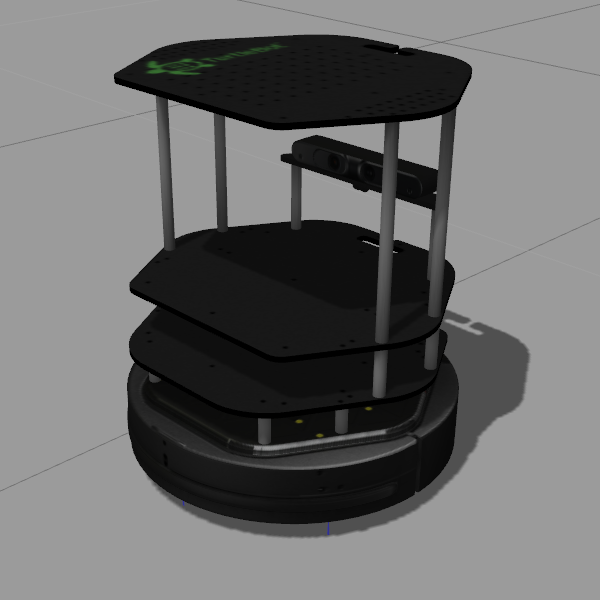
\includegraphics[width=.45\textwidth]{images/turtlebotsim_crop.png}
        \caption{Turtlebot model in Gazebo Simulator.}\label{fig:gazebo}
\end{figure}

We evaluate our approach by modeling the control policies for different Turtlebot systems \cite{Turtlebot-2016}. 
%Turtlebots are an affordable robotic platform that uses the Robotic Operating System (ROS) in its hydro version,
%which is compatible with the Gazebo simulator \cite{Gazebo-2016,ROS-2016}. 
Experiments were conducted using the Gazebo simulator \cite{Gazebo-2016,ROS-2016} with a simulated model of the Turtlebot as shown in Fig~\ref{fig:gazebo}. 
The implementation of our approach uses Python and the Hydro version of Robot Operating System (ROS).
This experimental setup allows us to use the same code in both simulation and the physical robots.

In a first attempt to explore disturbance rejection as a preamble of
fault tolerant control applications, the Turtlebot should learn how to drive itself from an initial point to a goal point.
%It should accomplish this simple task while being affected by a constant and unknown angular disturbance. 
We then artificially induce a random and constant disturbance to the control signal that is drawn uniformly from 
$[-0.1, 0.1] \subset \Re$ and measured in $m/s$. These limits were selected to provide a large noise that was still within the bounds of what the turtlebot accepts.
The disturbance now emulates a bias on the angular velocity of each robot that forces the robot to
compensate for the induced failure. It is worth mentioning that the difficulty of the disturbance can be increased by introducing
time varying disturbance and stochastic disturbances later on.


%The Gazebo simulator considers the kinematics and mechanics of the system. In a first attempt to explore disturbance rejection as a preamble of
%fault tolerant control applications, the Turtlebot should learn how to drive itself from an initial to a goal point.
%It should accomplish this simple task while being affected by a constant and unknown angular disturbance. Thus the robot is enforced to
%compensate for the induced failure. It is worth mentioning that the difficulty of the disturbance will be increased by assuming
%time varying disturbance and stochastic disturbances later on.

We assume we have little knowledge of the Turtlebot model, so we use the simplified kinematic model provided in \cite{aicardi1994closed}.
In the kinematic model, the state space is given by $\boldsymbol{x} \in \Re^3$ and the action space is described by 
$\boldsymbol{a} \in \Re^2$. Notice that the model in \cite{aicardi1994closed} just considers the kinematics of a unicycle in polar coordinates
so we do not consider the dynamics of the system, \emph{i.e.,} we are neglecting model parameters such as mass, damping and friction 
coefficients, as well as inputs such as forces and torques. Then, the nonlinear policy is derived neglecting the dynamics and just assuming
simple kinematics, therefore, taking into account that our action is given by 
$\boldsymbol{a} = \boldsymbol{\theta}^\transpose\boldsymbol{\phi}(\boldsymbol{x}) = (u,w)^\transpose$
where $\boldsymbol{x} = (\rho,\gamma,\psi)^\transpose$ as illustrated in Fig. \ref{fig:reward} we propose the following nonlinear gain vector
structure,

\begin{equation} \label{eqn:state}
	%\bm{x}^{(t)} \!=\! \begin{bmatrix} r cos(\alpha) & \alpha & \frac{cos(\alpha)sin(\alpha)}{\alpha}\left(\alpha + \kappa + \phi \right) & 1 \end{bmatrix} \enspace
	\boldsymbol{\phi}(\boldsymbol{x}) = \left(\begin{array}{c} \rho \cos(\gamma) \\ \gamma \\ \frac{\cos(\gamma)\sin(\gamma)}{\gamma}\left(\gamma + \psi \right) \\ 1 \end{array}\right) \enspace
\end{equation}
where $\rho$, $\gamma$ and $\psi$ are indicated in Fig. \ref{fig:numfeat}.



\begin{figure}[!htbp]
    \centering
        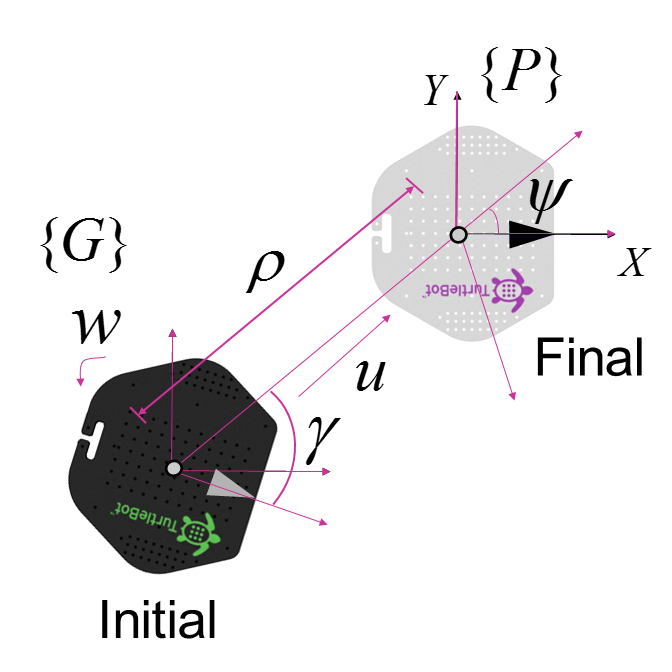
\includegraphics[width=.45\textwidth]{images/unicycle.png}
        \caption{State variables of simplified go-to-goal problem.}\label{fig:numfeat}
\end{figure}
The state is a non-linear transformation of the position and heading angle. We ran experiments using natural actor critic \cite{peters2008natural}, episodic REINFORCE \cite{williams1992simple}, and FD \cite{Bagnell-2013} and found FD to work best for our problem. We believe \comGabe{Is this speculating?} this is a result of the particular nonlinear transformation we are using and the fact that FD optimizes the true return. In future work we will present a comparison of different base learners. 

\subsection{Methodology}
We start by generating 20 robots, each with a different constant disturbance and a unique goal, both selected uniformly. 
We use 20 robots because it provides a large diversity in tasks but is a number that is still practical to run in simulation. 

To learn a controller for each task in RL, we use FD. Parameters are $\delta=1\times 10^{-6}$, $\gamma=0.9999$, and $\sigma=0.001$. 
Note that the same parameter values are used in PG-ELLA.\comGabe{not sure if sigma should be mentioned here because it's not mentioned in the algorithm section and should we add the noiseval here as well?}

FD is used to train each robot for 20 iterations with 15 roll-outs per iteration and 50 time-steps per roll-out.
%The robots are run for 20 learning steps of FD, each learning step consists of 15 roll-outs of 50 time steps each. 
Note that 20 learning steps is fewer iterations than is required for any system to converge to a good controller. 
The number of roll-outs and time steps were selected to allow for successful learning while minimizing the runtime. 
The policy that is learned after 20 iterations is used as $\theta^*$ for PG-ELLA. %We use a learning rate of $1\times 10^{-6}$. 

We learn our PG-ELLA knowledge repository $\bm{L}$ and sparse representation $\bm{s}^{(t)}$ using the update equations given 
by (\ref{onlineupdate}). Tasks are encountered randomly with repetition and learning stops once every task has been observed 
once. For our experiments we approximate the hessian with the identity matrix. For the parameters unique to PG-ELLA, we select $k=8$ to be the number of columns, and use sparsity coefficient $\mu = 1\times 10^{-3}$ and regularization coefficient $\lambda = 1\times 10^{-8}$. These coefficients were selected by trial and error. 

We then compare the policy reconstructed from PG-ELLA against the policy that was learned after 20 iterations of FD by comparing the learning curves that result from running FD for an additional 80 learning iterations. Performance is averaged over 6 trials for all 20 robots to increase our confidence in the results. In Figure \ref{fig:reward} we see that PG-ELLA is successfully able to reconstruct the policies and provide an additional benefit of positive transfer. We plot the change in reward of using PG-ELLA instead of PG in Figure \ref{fig:gain}, and observe that PG-ELLA improves the quality of the learned controllers. Note that these are preliminary results and we suspect further refinements will enable us to achieve larger amounts of transfer.

\begin{figure}[!htbp]
    \centering
        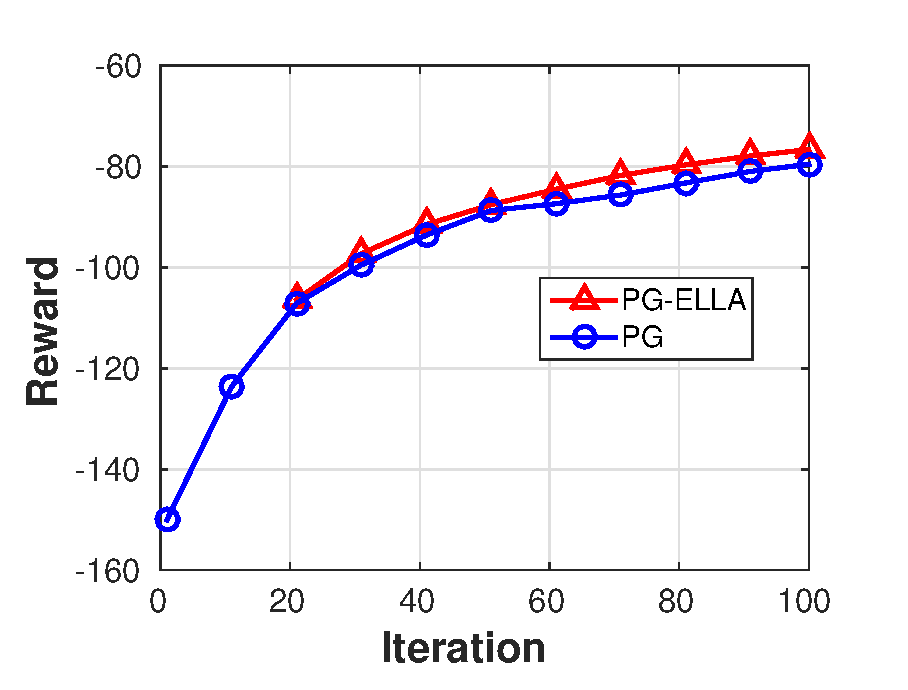
\includegraphics[width=.42\textwidth]{images/2016_02_06_learning.eps}
        \caption{Learning curves for FD and PG-ELLA using FD to transfer information between tasks. \comGabe{The legend on the figure should be FD instead of PG?} }\label{fig:reward}
\end{figure}

\begin{figure}[!htbp]
    \centering
        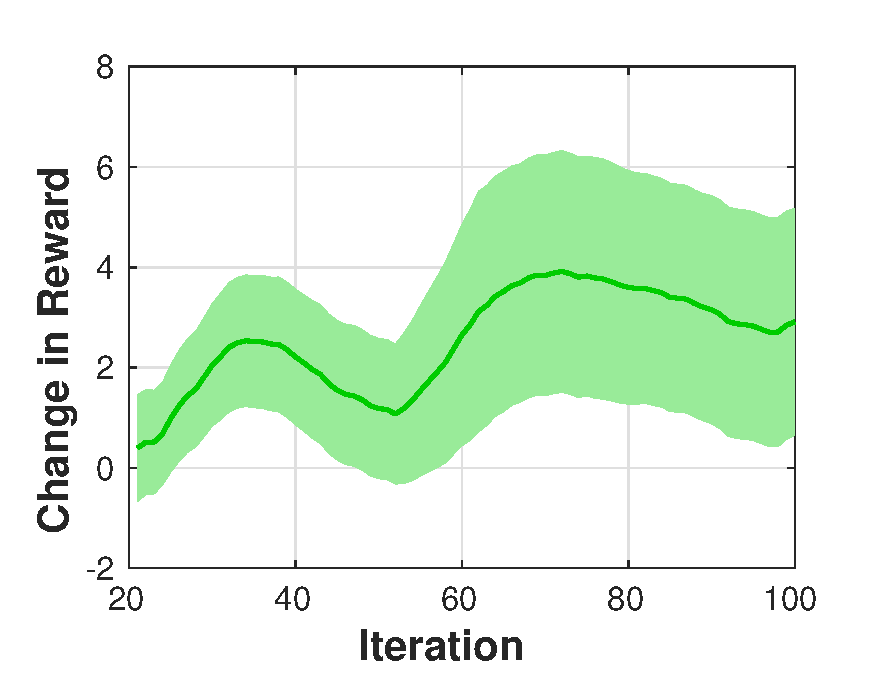
\includegraphics[width=.42\textwidth]{images/2016_02_06_gain.eps}
        \caption{The positive transfer achieved by using ELLA. }\label{fig:gain}
\end{figure}

\section{Conclusions}
We demonstrate the use of lifelong learning for disturbance rejection on Turtlebots. This is intended to lay the foundation for creating fault tolerant control on multi-agent systems. We show that PG-ELLA can be implemented on simulated turtlebots and that it outperforms standard PG. This suggests that PG-ELLA can be extended to real robotic systems.

%Acknowledgements are optional
\section*{Acknowledgments}
{\color{red} 
the grant goes here
}


\bibliographystyle{abbrv}
\bibliography{sigproc}  % sigproc.bib is the name of the Bibliography in this case
% You must have a proper ".bib" file
%  and remember to run:
% latex bibtex latex latex
% to resolve all references
%
% ACM needs 'a single self-contained file'!
%\balancecolumns % GM June 2007
% That's all folks!
\end{document}
